\documentclass[11pt]{article}

\usepackage[margin=1in]{geometry}
\usepackage[T1]{fontenc}
\usepackage[utf8]{inputenc}
\usepackage{lmodern}
\usepackage{graphicx}
\graphicspath{{./}{experiments/results/20261119_040644/}}
\usepackage{booktabs}
\usepackage{longtable}
\usepackage{array}
\usepackage{enumitem}
\usepackage{xcolor}
\usepackage[hidelinks]{hyperref}
\usepackage{caption}
\usepackage{float}
\usepackage{amsmath}
\usepackage{listings}

\lstset{
  basicstyle=\ttfamily\small,
  breaklines=true,
  frame=single,
  backgroundcolor=\color{gray!5},
  xleftmargin=1em,
  framexleftmargin=0.5em
}

\title{\textbf{RAG-based Question Answering over the Constitution of India}}
\author{
Prem Kumar \and Ritik Singh \and Satish Kumar \and Pooran Singh
}
\date{\textbf{Deep Learning Project}\\Instructor: Chhavi Sharma\\[0.5em]\today}

\begin{document}
\maketitle

\begin{abstract}
This project presents a retrieval-augmented question-answering system for the Constitution of India. The system combines an official Constitution corpus, Article-aware metadata extraction, dense vector retrieval, BM25 lexical retrieval, weighted Reciprocal Rank Fusion (RRF), a FastAPI backend, and a browser chat interface. A fixed set of 180 human-verified questions is used to compare no-retrieval, dense, BM25, and hybrid retrieval. On the archived evaluation run, hybrid retrieval achieved the best retrieval performance: Recall@5 = 0.741, Hit@5 = 0.756, and MRR = 0.598, compared with dense retrieval (0.666, 0.675, 0.538) and BM25 (0.659, 0.675, 0.547). The implementation also includes evidence-threshold abstention and citations constructed only from retrieved passage metadata. Reranking, RAGAS faithfulness and answer-relevance evaluation, and a configured LLM-without-retrieval baseline were not completed in the evaluated system. This report distinguishes implemented behaviour from planned extensions and reports the evidence exactly from the repository's archived run.
\end{abstract}

\section{Introduction}

Legal and constitutional text is dense, highly structured, and susceptible to misinterpretation. A conventional language model may answer a Constitution question fluently without being able to verify the claim against the authoritative text. A retrieval-augmented generation (RAG) system addresses this problem by retrieving relevant source passages before generating or presenting an answer \cite{Lewis2020}. It also provides a route for article-level citations and for abstaining when the retrieved evidence is insufficient.

The objective of this project was to build a chatbot that answers citizen questions grounded in the Constitution of India and cites the relevant Articles. The work proceeded from data ingestion and chunk construction to dense, lexical, and hybrid retrieval, before a small API and browser interface were added. The principal research question was:

\begin{quote}
\emph{Which retrieval design choices matter most for accurately locating and presenting supporting Constitution passages?}
\end{quote}

The study compared retrieval modes on a self-created 180-question test set. The completed evidence measures retrieval quality, not final answer quality. It is therefore explicitly reported that RAGAS \cite{Ragas2024} metrics were not available in the archived run.

\subsection{Project scope}

The working system includes:
\begin{itemize}[nosep]
  \item ingestion of the English Constitution PDF;
  \item Article and page metadata extraction;
  \item fixed-size, overlapping chunk construction;
  \item precomputed dense embeddings using \texttt{BAAI/bge-m3};
  \item BM25Okapi lexical retrieval;
  \item hybrid retrieval using Reciprocal Rank Fusion;
  \item evidence-sufficiency checking and abstention;
  \item citations resolved from retrieved chunk metadata;
  \item an OpenAI-compatible generation interface and an extractive baseline;
  \item FastAPI endpoints and a static chat interface.
\end{itemize}

The reranker, RAGAS-based final answer evaluation, and chunk-size experiments remain explicitly identified as future work rather than reported as completed features.

\section{Related Work}

Lewis et al.\ introduced retrieval-augmented generation as a method for grounding language models in external knowledge rather than relying exclusively on model parameters \cite{Lewis2020}. RAG separates knowledge storage and retrieval from text generation, making source traceability and corpus updates practical.

Dense retrieval encodes queries and passages into a shared embedding space. Lexical methods such as BM25 use term-frequency and inverse-document-frequency statistics and are especially effective for exact Article numbers and legal terminology. Hybrid systems combine both ranked lists, reducing the weaknesses of either method alone. RRF is one scale-free fusion method: it ranks items by reciprocal rank rather than by incompatible raw similarity scores.

RAGAS provides automatic framework metrics for retrieval-augmented answer quality, including faithfulness and answer relevance \cite{Ragas2024}. The project includes an optional RAGAS integration in the evaluation code, but the archived evaluation records that RAGAS was not run because no LLM generator was configured.

\section{Dataset and Corpus}

\subsection{Constitution source}

The source is the official Constitution of India PDF obtained from the Legislative Department of the Government of India. The repository records the source title, URL, source version, and PDF-derived metadata. The ingestion pipeline extracts text, cleans extraction artefacts, parses Article records, and creates stable chunks.

\subsection{Chunk construction}

The current corpus is built with a character limit of 1200 and an overlap of 200 characters. Article text is split at word boundaries while preserving Article number, title, page range, and source metadata. Schedules and appendices after the Article section are represented as page-scoped supplement chunks.

The resulting archived corpus contains 953 chunks. Its SHA-256 is
\texttt{3fffae984ed5472321bac46b773ad11def8dcafa11dda6cdeed3c485be0017fc}.
The embedding file contains 953 vectors of dimension 1024 using
\texttt{BAAI/bge-m3}.

\subsection{Question-answer test set}

The evaluation dataset contains 180 human-verified questions. It has 160 answerable questions and 20 out-of-corpus, unanswerable questions. The dataset is divided into development and held-out test splits of 48 and 132 questions. It includes six categories:
\begin{itemize}[nosep]
  \item direct Article questions;
  \item paraphrased questions;
  \item keyword-heavy questions;
  \item multi-Article questions;
  \item ambiguous questions;
  \item out-of-corpus questions.
\end{itemize}

Each row stores a reference answer, relevant Articles, evidence chunk IDs, answerability, category, split, and review status. The dataset SHA-256 is
\texttt{929a78f1f39f793c336c731ec09fdaf922673e89361c7260346bfe1a4983f092}.

\section{System Architecture}

\subsection{Offline ingestion}

The offline pipeline is:
\[
\text{Official PDF}
\rightarrow \text{text extraction}
\rightarrow \text{cleaning}
\rightarrow \text{Article parsing}
\rightarrow \text{chunking}
\rightarrow \text{embedding corpus}
\]

The final corpus and embedding records are JSON Lines files. Stable chunk IDs such as \texttt{article\_14\_chunk\_0} enable retrieval results to be linked to source metadata.

\subsection{Online question-answering pipeline}

The online pipeline performs the following operations:
\begin{enumerate}[nosep]
  \item validate the question and retrieval mode;
  \item retrieve top-$k$ passages;
  \item compare the top passage score with an evidence threshold;
  \item abstain or pass the passages to a generation service;
  \item construct citations only from retrieved chunk metadata;
  \item return the answer, citations, sources, and status to the UI.
\end{enumerate}

The FastAPI application exposes \texttt{GET /health} and \texttt{POST /ask}. It accepts \texttt{dense}, \texttt{bm25}, or \texttt{hybrid}. Requests are limited to 1000 characters. If a retrieval backend or provider is unavailable, the API returns a structured 503 or provider error instead of silently changing strategy.

\subsection{Generation and abstention}

The extractive baseline surfaces the top retrieved passage verbatim and labels itself as extractive. This baseline is deliberately non-generative and cannot create a model-authored constitutional claim. An OpenAI-compatible generator can be configured for a provider, model, and base URL; it receives retrieved passages and is instructed not to invent Article numbers or citations.

Citation metadata is not trusted to the generator. The orchestrator creates \texttt{Citation} objects from \texttt{RetrievedPassage.chunk} fields. This prevents the language model from introducing a citation ID that was not retrieved.

\section{Retrieval Methods}

\subsection{Dense retrieval}

The dense retriever loads precomputed normalized \texttt{bge-m3} embeddings and encodes the question with the same model. Cosine similarity is computed by a dot product of normalized vectors. A fixed top-$k=5$ ranking is returned. The retriever has no fallback to another backend.

\subsection{BM25 retrieval}

BM25Okapi provides the lexical baseline. Text is lowercased and tokenized into alphanumeric terms, while numbers are preserved so queries such as ``Article 21'' retain numeric information. Article references in a question also trigger a corpus-level boost for chunks whose Article number matches. This is a lexical domain enhancement, not a reranker.

\subsection{Hybrid retrieval}

The hybrid retriever obtains dense and BM25 candidates independently, then applies RRF:
\[
\mathrm{RRF}(c)=
\sum_{m\in\{\mathrm{dense},\mathrm{bm25}\}}
\frac{w_m}{k_{\mathrm{RRF}}+\mathrm{rank}_m(c)}
\]

The archived run used equal weights, \texttt{rrf\_k=60}, and top-$k=5$. RRF avoids combining cosine scores, unbounded BM25 scores, and RRF scores directly.

\subsection{Deferred reranker and chunk study}

A reranker layer was part of the intended design but was not implemented in the evaluated system (\texttt{RERANKER\_ENABLED=false}). Similarly, no multiple-chunk-size comparison was completed in the archived evidence. The report therefore makes no unsupported claim that reranking or another chunk size improves this system.

\section{Evaluation Methodology}

\subsection{Metrics}

For answerable questions, Recall@k measures overlap with gold evidence:
\[
\mathrm{Recall@k}
=\frac{|\mathrm{top}\text{-}k\ retrieved \cap gold|}
{|\mathrm{gold}|}
\]

Hit@k indicates whether at least one gold chunk appears in the top-$k$ list. MRR is the mean reciprocal rank of the first gold chunk. Context precision is the fraction of the retrieved set that overlaps gold evidence. Citation accuracy in this harness checks whether citations refer to retrieved chunk IDs, not whether text semantically supports a claim.

\subsection{Experimental controls}

The same 180 questions and corpus were used across modes. The only retrieval mechanism changed from run to run. The result manifest records run ID, timestamps, corpus and dataset hashes, embedding model, chunk settings, top-$k$, hybrid parameters, environment, and package versions.

\subsection{Evidence-threshold calibration}

A top-1 score threshold is used to decide whether the evidence is sufficient. The development set is used for Youden's J selection:
\[
J=\mathrm{answerable\ retention}-\mathrm{unanswerable\ answer\ rate}
\]

The selected threshold is then confirmed on the held-out test set. Because dense, BM25, and hybrid scores occupy incompatible ranges, one shared threshold is not appropriate.

\section{Experimental Results}

\subsection{Overall retrieval performance}

Table~\ref{tab:main-results} reports the main run.

\begin{table}[H]
\centering
\caption{Retrieval performance for the archived run \texttt{20261119\_040644}.}
\label{tab:main-results}
\begin{tabular}{lrrrrrrr}
\toprule
Mode & $n$ & Recall@5 & Hit@5 & MRR & Context precision & Context recall & Latency (ms) \\
\midrule
No retrieval & 180 & 0.000 & 0.000 & 0.000 & 0.000 & 0.000 & n/a \\
Dense & 180 & 0.666 & 0.675 & 0.538 & 0.143 & 0.666 & 1561 mean \\
BM25 & 180 & 0.659 & 0.675 & 0.547 & 0.139 & 0.659 & 20 mean \\
Hybrid & 180 & \textbf{0.741} & \textbf{0.756} & \textbf{0.598} & \textbf{0.156} & 0.741 & 967 mean \\
\bottomrule
\end{tabular}
\end{table}

Hybrid retrieval performed best in Recall@5, Hit@5, MRR, and context precision. It improved Recall@5 by 7.5 percentage points over dense retrieval and 8.1 percentage points over BM25. BM25 was fastest, while dense retrieval was the slowest. Hybrid retrieval reduced BM25 latency while improving quality.

\subsection{Performance by category}

\begin{table}[H]
\centering
\caption{Category-level recall and Hit@5.}
\label{tab:category-results}
\begin{tabular}{lrrrrrrr}
\toprule
Category & $n$ & Dense R & Dense H & BM25 R & BM25 H & Hybrid R & Hybrid H \\
\midrule
Direct Article & 45 & 0.200 & 0.200 & 0.156 & 0.156 & 0.244 & 0.244 \\
Paraphrased & 45 & 0.889 & 0.889 & 0.844 & 0.844 & 0.933 & 0.933 \\
Keyword-heavy & 45 & 0.800 & 0.800 & 0.978 & 0.978 & 1.000 & 1.000 \\
Multi-Article & 15 & 0.900 & 1.000 & 0.767 & 0.933 & 0.833 & 1.000 \\
Ambiguous & 10 & 0.800 & 0.800 & 0.500 & 0.500 & 0.800 & 0.800 \\
Unanswerable & 20 & 0.000 & 0.000 & 0.000 & 0.000 & 0.000 & 0.000 \\
\bottomrule
\end{tabular}
\end{table}

Hybrid retrieval won overall and in every category except multi-Article recall, where dense retrieval scored 0.900 compared with hybrid 0.833; both achieved Hit@5 = 1.000.

\subsection{Threshold calibration}

\begin{table}[H]
\centering
\caption{Per-mode score thresholds selected on development data and confirmed on test data.}
\label{tab:threshold}
\begin{tabular}{lrrrrrrr}
\toprule
Mode & Threshold & Dev retention & Dev abstention & Dev J & Test retention & Test abstention & Test J \\
\midrule
Dense & 0.5576 & 0.884 & 1.000 & 0.884 & 0.829 & 1.000 & 0.829 \\
BM25 & 24.7565 & 0.279 & 1.000 & 0.279 & 0.453 & 1.000 & 0.453 \\
Hybrid & 0.0321 & 0.698 & 0.600 & 0.298 & 0.590 & 0.733 & 0.323 \\
\bottomrule
\end{tabular}
\end{table}

The BM25 and hybrid thresholds demonstrate why a common 0.6 threshold is unsafe. BM25 scores are unbounded and roughly in the range 9--76, whereas hybrid RRF scores are roughly 0.016--0.033. The shipped value 0.6 would effectively allow every BM25 result and always abstain for hybrid retrieval. The calibrated values are recommendations and were not silently applied to the API.

\begin{figure}[H]
\centering
\IfFileExists{score_distributions.png}{
  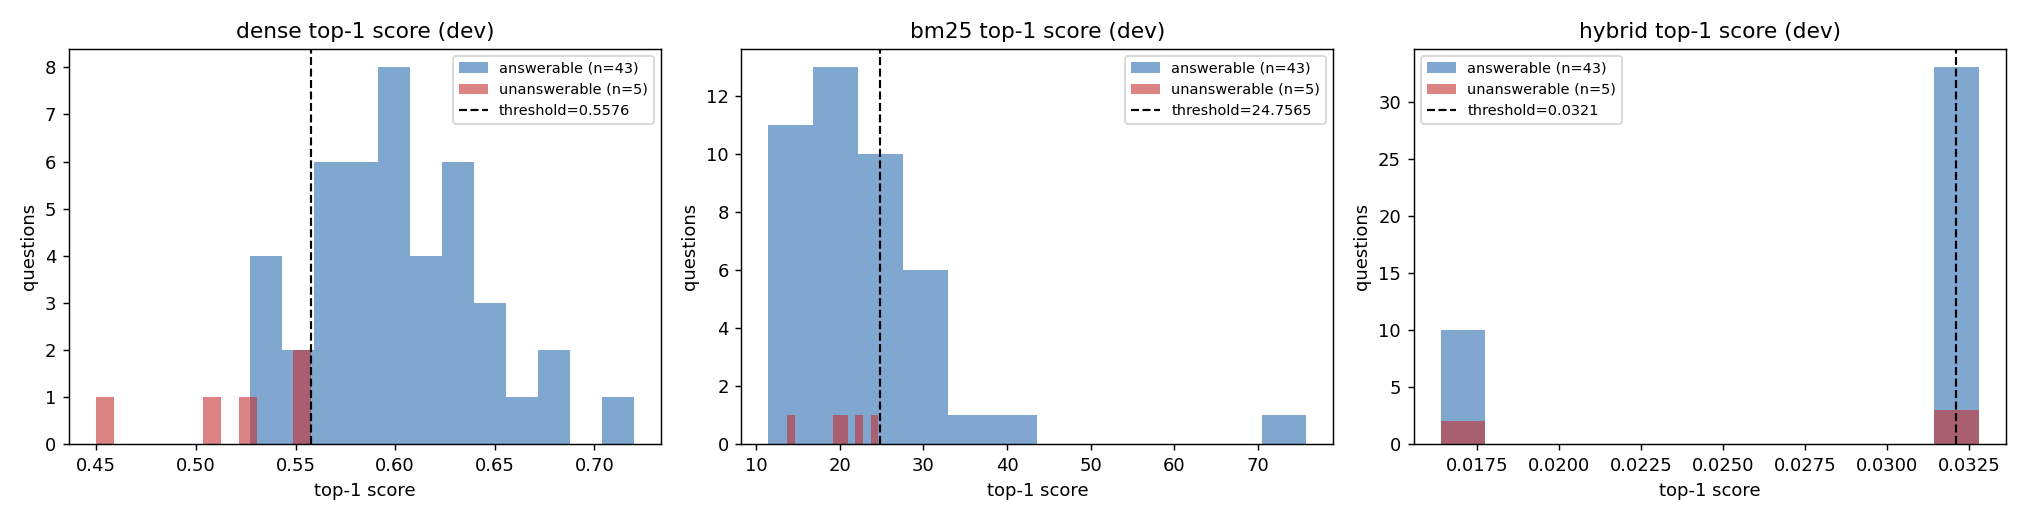
\includegraphics[width=0.82\textwidth]{score_distributions.png}
}{
  \fbox{\parbox{0.8\textwidth}{\centering
    Figure not found. Upload \texttt{score\_distributions.png} to the
    Overleaf project root, or upload the archived results folder.}}
}
\caption{Answerable and unanswerable top-1 score distributions from the archived run.}
\label{fig:scores}
\end{figure}

\section{Failure Analysis}

\subsection{Fixed-size chunking}

The dominant retrieval weakness was the fixed character-size chunking policy. A chunk often contains several Articles and some chunks do not carry reliable Article metadata. This caused direct Article questions to retrieve sections from neighbouring Articles or from the table of contents.

Direct Article recall was low for dense (0.200), BM25 (0.156), and hybrid (0.244). The result set showed 52 dense misses, 52 BM25 misses, and 39 hybrid misses among the 160 answerable questions.

\subsection{Article metadata limitations}

The evaluated corpus has Article-aware chunking for the Article section, but the current final report notes that Article/page/source values are incomplete for some records and the strict gold evidence remains based on chunk IDs. The citation accuracy metric reached 1.000, but this only confirms that cited IDs come from retrieved passages. It does not measure whether the answer semantically matches the passage.

\subsection{Abstention trade-off}

Dense calibration retained 82.9 percent of test answerable questions and abstained for all 15 test unanswerable questions. BM25 retained only 45.3 percent of test answerable questions but abstained for all unanswerable questions. Hybrid retained 59.0 percent and abstained for 73.3 percent of unanswerable questions, while still producing false answers for six unanswerable questions in the overall set. Calibration trades answer retention against unsupported answers.

\section{User Interface and API}

The static browser interface communicates with \texttt{/ask}, displays loading, success, insufficient-evidence, and error states, and separates the answer from supporting passages. It gives a clear notice that the system is for educational purposes and does not provide legal advice.

The backend is provider-neutral: \texttt{GenerationService} is an interface implemented by both an extractive baseline and an OpenAI-compatible generator. It also supports health reporting and degraded operation when local artifacts or models are unavailable.

\section{Limitations}

\begin{enumerate}[nosep]
  \item RAGAS faithfulness and answer relevance were not run.
  \item The reranker was not implemented.
  \item Only one 1200-character chunk size and 200-character overlap were evaluated in the main archived run.
  \item The single human verification workflow has no inter-annotator agreement estimate.
  \item The unanswerable development set is small: five questions.
  \item Strict chunk-ID gold evidence may penalise retrieval of a different chunk for the same Article.
  \item Latency is retrieval-only and CPU-only; end-to-end generation latency was not measured.
  \item Context precision is low because a small gold evidence set is compared with five retrieved passages.
  \item Citation accuracy is structural and should not be interpreted as semantic citation correctness.
\end{enumerate}

\section{Future Work}

\begin{enumerate}[nosep]
  \item Replace fixed character chunks with clause- and paragraph-aware Article chunks.
  \item Extend and validate Article metadata across the complete corpus.
  \item Add a bounded reranker and compare it with dense, BM25, and hybrid retrieval.
  \item Study chunk sizes and overlaps on a held-out development set.
  \item Calibrate per-mode thresholds and expose the selected threshold through configuration.
  \item Configure an LLM provider and run RAGAS faithfulness and answer relevance.
  \item Measure answer correctness by human evaluation and multi-annotator review.
  \item Compare additional embedding models and a FAISS-backed ANN index if the corpus grows.
\end{enumerate}

\section{Conclusion}

This project implements a complete Constitution RAG workflow from an official corpus through retrieval, abstention, citations, API delivery, and a browser interface. In the archived evaluation, the hybrid RRF retriever was the strongest retrieval system, improving Recall@5 from 0.666 (dense) and 0.659 (BM25) to 0.741.

The results also identify fixed-size chunking and Article metadata as the most important remaining retrieval limitation. BM25 is useful for exact terms and Article numbers, while dense retrieval handles semantic paraphrases. Hybrid fusion combines these strengths. However, retrieval quality is not answer quality: RAGAS and final generation metrics remain to be completed, and the reranker and chunk-size studies are future work.

\section*{Acknowledgements}

The team ownership in the repository is: Prem Kumar for corpus ingestion and embeddings; Ritik Singh for the backend API and chat UI; Satish Kumar for retrieval experiments and evaluation; and Pooran Singh for the QA dataset and planned generator fine-tuning.

\begin{thebibliography}{9}

\bibitem{Lewis2020}
P.~Lewis, E.~Perez, A.~Piktus, F.~Petroni, V.~Karpukhin, N.~Goyal,
H.~K\"uttler, M.~Lewis, W.-t.\ Yih, T.~Rockt\"aschel, S.~Riedel, and
D.~Kiela.
\newblock Retrieval-Augmented Generation for Knowledge-Intensive NLP Tasks.
\newblock In \em{Advances in Neural Information Processing Systems},
2020.
\newblock \url{https://arxiv.org/abs/2005.11401}

\bibitem{Ragas2024}
S.~Es, J.~James, L.~Espinosa-Anke, and S.~Schockaert.
\newblock RAGAS: Automated Evaluation of Retrieval Augmented Generation.
\newblock In \em{Proceedings of the EACL 2024 System Demonstrations},
2024.
\newblock \url{https://arxiv.org/abs/2309.15217}

\bibitem{OfficialConstitution}
Legislative Department, Government of India.
\newblock \em{The Constitution of India}.
\newblock Official English text.
\newblock \url{https://legislative.gov.in/constitution-of-india/}

\bibitem{BgeM3}
J.~Chen, S.~Chen, H.~He, Z.~Li, X.~Mao, Y.~Chen, and T.~Li.
\newblock BGE M3-Embedding: Multi-Lingual, Multi-Functionality,
Multi-Granularity Text Embeddings.
\newblock 2024.
\newblock \url{https://huggingface.co/BAAI/bge-m3}

\end{thebibliography}

\end{document}
